\section{Estructura de los modelos matemáticos}
\label{sec:formulations}

\begin{frame}{Estructura De Un Modelo Matemático}

Todos los modelos de IO, incluido el de Programación Lineal (PL), constan de tres componentes básicos.

  \begin{enumerate} \justifying 
  \item Los \alert{parámetros} o variables externas que no están bajo nuestro control.
  \item Las \alert{variables de decisión} que pretendemos determinar.
  \item El \alert{objetivo} (la meta) que necesitamos optimizar (maximizar o minimizar).
  \item Las \alert{restricciones} que la solución debe satisfacer.
  \end{enumerate}
   
\end{frame}

\begin{frameExample}{1}{}
  \only<1>{%
    Reddy Mikks produce pinturas para interiores y exteriores con dos materias primas, $M_1$ y $M_2$. La tabla siguiente proporciona los datos básicos del problema. Una encuesta de mercado indica que la demanda diaria de pintura para interiores no puede exceder la de pintura para exteriores en más de una tonelada. Asimismo, que la demanda diaria máxima de pintura para interiores es de dos toneladas. Reddy Mikks se propone determinar la (mejor) combinación óptima de pinturas para interiores y exteriores que maximice la utilidad diaria total.%
  }


  {\centering
  \includegraphics<1>[scale=0.6]{reddy-mikks_01}
  \par}
\end{frameExample}



%%% Local Variables:
%%% mode: latex
%%% TeX-master: "../slides"
%%% End:

\begin{frameExample}{Producción}{}
  % EXAMPLE 2.6-1 (Production Allocation Problem} Gupta ebook
  Una empresa produce tres productos. Estos productos se procesan en tres máquinas diferentes. El tiempo requerido para fabricar una unidad de cada uno de los tres productos y la capacidad diaria de las tres máquinas se detallan en la tabla a continuación.

  {\centering
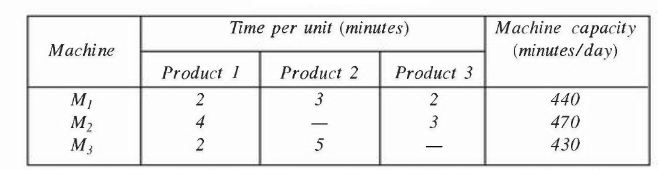
\includegraphics[scale=0.5]{example_allocation_gupta}
\par}

   Se requiere determinar la cantidad diaria de unidades que se fabricarán para cada producto. El beneficio por unidad para el producto 1, 2 y 3 es de \$ 4, \$ 3 y \$ 6 respectivamente. Se supone que todas las cantidades producidas se consumen en el mercado. Formule el modelo matemático (L.P.) que maximizará la ganancia diaria.
\end{frameExample}



%%% Local Variables:
%%% mode: latex
%%% TeX-master: "../slides"
%%% End:

\begin{frameExample}{Dieta}{}
  % EXAMPLE 2.6-2 {Diet Problem} Gupta
  La persona quiere decidir los componentes de una dieta que cumpla con sus requerimientos diarios de proteínas, grasas y carbohidratos al costo mínimo. La elección debe hacerse a partir de cuatro tipos diferentes de alimentos. Los rendimientos por unidad de estos alimentos se dan en la tabla siguiente. Formule un modelo de programación lineal para el problema.
  
  {\centering
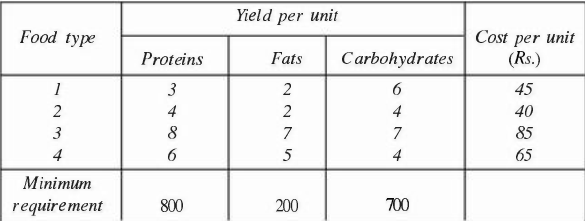
\includegraphics[scale=0.5]{example_diet_gupta}
\par}

  
\end{frameExample}



%%% Local Variables:
%%% mode: latex
%%% TeX-master: "../slides"
%%% End:

\begin{frameExample}{Mezcla}{}
  % EXAMPLE 2.6-3 (Blending Problem) 
  \only<1>{%
    Una empresa produce una aleación que tiene las siguientes especificaciones:

\begin{enumerate}[i)]  \justifying
\item  gravedad específica $\leq$ O. 98,
\item  cromo $\geq$ 8\%,
\item  punto de fusión $\geq$ 450°C.
\end{enumerate}

Las materias primas A, B y C que tienen las propiedades que se muestran en la tabla pueden usarse para hacer la aleación.%
}

  {\centering
\includegraphics<1,2>[scale=0.5]{example_blending_gupta}
\par}

\only<2>{Los costos de las diversas materias primas por tonelada son: \$ 90 para A, \$ 280 para B y \$ 40 para C. Formule el modelo L.P. para encontrar las proporciones en las que se utilizarán A, B y C para obtener una aleación de las propiedades deseadas, mientras que el costo de las materias primas es mínimo.}
    
\end{frameExample}



%%% Local Variables:
%%% mode: latex
%%% TeX-master: "../slides"
%%% End:

\begin{frameExample}{Seleccion de Medios}{}
  % LE 2.6-4 (Advertising Media Selection Problem) 

  \only<1>{%
  Una empresa de publicidad desea planificar su estrategia publicitaria en tres medios diferentes de televisión, radio y revistas. El objetivo de la publicidad es llegar al mayor número posible de clientes posibles. Se han obtenido los siguientes datos de una encuesta de mercado:%
  }

    {\centering
\includegraphics<1,2>[scale=0.5]{example_selection-media_gupta}
\par}

\only<2>{%
La compañía quiere gastar no más de \$ 450,000 en publicidad. Los siguientes son los requisitos adicionales que deben cumplirse:
\begin{enumerate}[i)] \justifying
\item  se producen al menos 1 millón de exposiciones entre clientes femeninas,
\item  la publicidad en revistas se limitará a \$ 150,000
\item  se deben comprar al menos 3 unidades publicitarias en la revista I y 2 unidades en la revista
\item  el número de unidades publicitarias en televisión y radio debe ser 5 y 10 cada uno.
\end{enumerate}

Formular un modelo L.P. para el problema.%
}
    
\end{frameExample}



%%% Local Variables:
%%% mode: latex
%%% TeX-master: "../slides"
%%% End:

\begin{frameExample}{Inspección}{}
  % EXAMPLE 2.6-5 {lnspection Problem} Gupta
Una empresa tiene dos grados de inspectores, I y II para llevar a cabo la inspección de control de calidad. Se deben inspeccionar al menos 1,500 piezas en un día de 8 horas. El inspector de grado I puede verificar 20 piezas en una hora con una precisión del 96\%. Grado II el inspector verifica 14 piezas por hora con un precisión del 92\%. Los salarios del inspector de grado I son \$ 5 por hora, mientras que los de grado II inspector son \$ 4 por hora. Cualquier error cometido por un inspector cuesta \$ 3 a la empresa. Si hay, en total, 10 grado I
inspectores y 15 inspectores de grado II en la empresa, encuentre la asignación óptima de inspectores que minimiza el costo diario de inspección.
    
\end{frameExample}



%%% Local Variables:
%%% mode: latex
%%% TeX-master: "../slides"
%%% End:

\begin{frameExample}{Mezcla de Productos}{}
  % EXAMPLE 2.6-6 (Product Mix Problem) Gupta
Una compañía química produce dos productos, $X$ e $Y$. Cada unidad de producto $X$ requiere 3 horas en operación I y 4 horas en operación II, mientras que cada unidad de producto $Y$ requiere 4 horas en operación I y 5 horas en operación II. El tiempo total disponible para las operaciones I y II es 20 horas y 26 horas respectivamente. La producción de cada unidad de producto $Y$ también da como resultado dos unidades de un subproducto $Z$ sin costo adicional. El producto $X$ se vende con una ganancia de \$ 10 / unidad, mientras que $Y$ se vende con una ganancia de \$ 20 / unidad. El subproducto $Z$ aporta un beneficio unitario de \$ 6 si se vende; en caso de que no se pueda vender, el costo de destrucción es de \$ 4 / unidad. Los pronósticos indican que no se pueden vender más de 5 unidades de $Z$. Formule el modelo L.P. para determinar las cantidades de $X$ e $Y$ que se producirán, teniendo en cuenta $Z$, de modo que la ganancia obtenida sea máxima.
    
\end{frameExample}



%%% Local Variables:
%%% mode: latex
%%% TeX-master: "../slides"
%%% End:

\begin{frameExample}{Mezcla de Productos (Fracciones)}{}
  % EXAMPLE 2.6-7 (Product Mix Problem) Gupta
Una empresa fabrica tres productos A, B y C. El tiempo para fabricar el producto A es el doble que para B y tres veces para C y si toda la mano de obra se dedica a la fabricación del producto A, se pueden producir 1,600 unidades de este producto. Estos productos deben producirse en una proporción de 3: 4: 5. Hay demanda de al menos 300, 250 y 200 unidades de productos A, B y C y el beneficio obtenido por unidad es de \$ 90, \$ 40 y \$ 30 respectivamente. Formule el problema como un problema de programación lineal.

{\centering
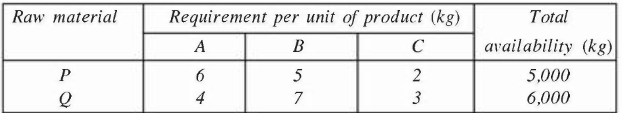
\includegraphics[scale=0.5]{example_product-mix02_gupta}
\par}

\end{frameExample}



%%% Local Variables:
%%% mode: latex
%%% TeX-master: "../slides"
%%% End:

\begin{frameExample}{Corte de Papel}{}
  % EXAMPLE 2.6-8 (Trim Loss Problem} 
  \only<1>{%
Una fábrica de papel produce rollos de papel utilizados para hacer cajas registradoras. Cada rollo de papel tiene una longitud de 100 m y se puede utilizar en anchos de 3, 4, 6 y 10 cm. El proceso de producción de la compañía da como resultado rollos de 24 cm de ancho. Por lo tanto, la empresa debe cortar su rollo de 24 cm al ancho deseado. Tiene seis alternativas básicas de corte de la siguiente manera:%
  }

  \begin{onlyenv}<1>
      {\centering
    \scalebox{0.7}{%
      \begin{tabular}{cccccc}
        \toprule
        Alternativas&\multicolumn{4}{c}{Ancho de los}&\\
        de corte&\multicolumn{4}{c}{rollos (cm)}&Desperdicio (cm)\\
        \cmidrule{2-5}
                    &3&4&6&10&\\
        \midrule[0.4pt]
        1&4&3&--&--&--\\
        2&--&3&2&--&--\\
        3&1&1&1&1&1\\
        4&--&--&2&1&2\\
        5&--&4&1&--&2\\
        6&3&2&1&--&1\\
        \bottomrule
      \end{tabular}
    }% \scalebox
% \includegraphics<1>[scale=0.5]{example_trim-loss_gupta}
\par}
  \end{onlyenv}

\only<2>{%
  La demanda mínima para los cuatro rollos es la siguiente:
  
{\centering
  \scalebox{0.8}{%
  \begin{tabular}{cr}
    \toprule
    Ancho del rollo (cm) & Demanda\\
     \midrule
    2 & 2,000 \\
    4 &3,600 \\
    6 &1,600 \\
    10 &500\\
    \bottomrule
  \end{tabular}
  }
  \par}

La fábrica de papel desea minimizar el desperdicio resultante del recorte al tamaño. Formule el modelo L.P.%
}

\end{frameExample}



%%% Local Variables:
%%% mode: latex
%%% TeX-master: "../slides"
%%% End:

\begin{frameExample}{Planeación de la Producción}{}
  % EXAMPLE 2.6-9 (Production Planning Problem) 
Una fábrica elabora un producto cuya unidad consta de 5 unidades de la parte A y 4 unidades de la parte B. Las dos partes A y B requieren diferentes materias primas, de las cuales están disponibles 120 unidades y 240 unidades respectivamente. Estas piezas pueden fabricarse por tres métodos diferentes. Los requisitos de materia prima por producción y el número de unidades para cada parte producida se detallan a continuación. Formule el modelo L.P. para determinar el número de corridas de producción para cada método a fin de maximizar el número total de unidades completas del producto final.

{\centering
%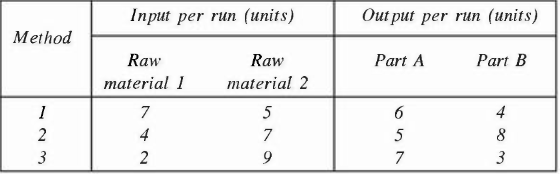
\includegraphics[scale=0.5]{example_production-planning_gupta}
  \scalebox{0.7}{%
    \begin{tabular}{ccccc}
      \toprule
  &\multicolumn{2}{c}{Entrada Por Corrida (unidades)}&\multicolumn{2}{c}{Salidas Por Corrida (unidades)}\\
  \cmidrule{2-5}
  Método&Materia & Materia & Parte&Parte \\
        &prima 1& prima 2&A&B\\
  \midrule
  1&7 &5 &6& 4\\
  2&4&7&5&8\\
  3&2&9&7&3\\
  \bottomrule
\end{tabular}
  } % \scalebox
\par}
\end{frameExample}

\begin{frameExample}{Planeación de la Producción}{}
  La función objetivo a maximizar es  \[ Z = \min \left(  \frac{6x_1 + 5x_2 + 7x_3}{5}, \frac{4x_1 + 8x_2 + 3x_3}{4}\right ) \]
  Las restricciones de disponibilidad de materias primas son:
  \begin{flalign*}
    7x_1 + 4x_2 +2x_3 &\leq 120\\
    5x_1 + 7x_2 +9x_3 &\leq 240\\
  \end{flalign*}
  La formulación anterior viola las propiedades de un programa lineal porque el objetivo es una función no lineal. El modelo se puede transformar a su versión equivalente lineal de la siguiente manera. 
  \[ y =  \min \left(  \frac{6x_1 + 5x_2 + 7x_3}{5}, \frac{4x_1 + 8x_2 + 3x_3}{4}\right )\]
  
\end{frameExample}

\begin{frameExample}{Planeación de la Producción}{}
  Tenemos entonces que
  \begin{flalign*}
    \frac{6x_1 + 5x_2 + 7x_3}{5} & \geq y\\
    \frac{4x_1 + 8x_2 + 3x_3}{4} & \geq y
  \end{flalign*}

  Por lo que el modelo matemático es:
\[ \max Z = y \]
sujeto a (s.t.)
  \begin{columns}[t]
    \column{0.4\textwidth}
\begin{flalign*}
    7x_1 + 4x_2 + 2x_3 & \leq 120\\
    5x_1 + 7x_2 + 9x_3 & \leq 240\\
  \end{flalign*}
  \column{0.4\textwidth}
    \begin{flalign*}
    6x_1 + 5x_2 + 7x_3 - 5y & \geq 0\\
    4x_1 + 8x_2 + 3x_3 - 4y & \geq 0\\
  \end{flalign*}
  \end{columns}
$x_1, x_2, x_3, y   \geq 0 $
\end{frameExample}
%%% Local Variables:
%%% mode: latex
%%% TeX-master: "../slides"
%%% End:



%%% Local Variables:
%%% mode: latex
%%% TeX-master: "slides"
%%% End:
